\documentclass[fleqn]{jbook}
\usepackage{physpub}

\begin{document}

\begin{question}{専攻 問題2}{}

一様な磁場の中に置かれた強磁性体の、次のような模型を考える。

3次元立方格子の各格子点$i$に磁気モーメント$\sigma _{i}$が存在し、
その磁場方向の成分は、$\sigma _{i} = +1$または$\sigma _{i} = -1$
の離散的な値をとる。隣り合う格子点$i$、$j$の磁気モーメントは、
相互作用のエネルギー$-J\sigma _{i}\sigma _{j}$($J$は正の定数)
を持つ。磁場を$h$とするとき、系のハミルトニアンは、
\[
H = -J \sum_{(i,j)}\sigma _{i}\sigma _{j} - h \sum_{i}\sigma _{i}
\]
で与えられる。ここで和$(i,j)$は最近接の格子点の間のみを
とるものとし、3次元立方格子のサイズは十分に大きいものとする。

\begin{subquestions}
\SubQuestion
系の温度を$T$として、以下の問に答えよ。

\begin{subsubquestions}
\SubSubQuestion
$T \rightarrow 0$および$T \rightarrow \infty$の極限における、
系の磁気モーメントの配位の様子を述べよ。

\SubSubQuestion
同じく$T \rightarrow 0$および$T \rightarrow \infty$の極限における、
1格子点あたりのエントロピーを求めよ。

\SubSubQuestion
(i)の結果を、自由エネルギー$F(T)$の振る舞いにより説明せよ。 

\end{subsubquestions}

\SubQuestion
磁気モーメントの熱力学的平均を近似的に求める
(厳密解は求められていない)。そのため、原点の磁気モーメント
$\sigma _{0}$とその最近接格子点の磁気モーメントからなる
部分系を考え、そのハミルトニアンを$H(\sigma _{0})$とする。

\begin{subsubquestions}
\SubSubQuestion
$H(\sigma _{0})$において、原点以外の格子点の磁気モーメントを
近似的に定数$m$で置き換える。このとき、$H(\sigma _{0})$
によって決まる、磁気モーメントの熱力学的平均$\langle \sigma _{0} \rangle $
を求めよ。

\SubSubQuestion
$\langle \sigma _{0}\rangle $を$m$に等しいと置く事により、$m$の満たす
方程式を求めよ。

\SubSubQuestion
磁場が0(すなわち$h = 0$)のとき、$m$を温度$T$の関数として
定性的にグラフに書け。ここで設問1{\bf (i)}の結果を考慮すること。

\SubSubQuestion
$m(T)$が特異点となる温度$T_c$を求めよ。

\end{subsubquestions}
\end{subquestions}
\end{question}
\begin{answer}{専攻 問題2}{}
\begin{subanswers}
\SubAnswer \begin{subsubanswers} 

\SubSubAnswer 

$T \rightarrow 0$では
  $J>0$より、すべての磁気モーメントが同じ向きを向く向きでは磁場の向き
  \\ 
$T \rightarrow \infty$では、バラバラの向きを向く。\\ 
($1$と$-1$は同じ数) 

\SubSubAnswer


全エントロピーは場合の数を$W$とすると
  $S=k \ln W$より、$N$粒子とすると$T \rightarrow 0$では状態は一つに定
  まり$S=0$。よって、$\frac{S}{N}=0$\\ $T \rightarrow \infty$では、
  Steringの公式を用いて(但し$N$は十分大とする。)、

\[ S= \ln _N
  C_{\frac{N}{2}}=k \left( \ln N! - 2 \ln \left( \frac{N}{2}! \right)
  \right) \simeq Nk \ln 2 
\]
よって$\frac{S}{N}=k \ln 2$ \SubSubAnswer
  $F=U-TS$を最小にする状態が実現され、各々の極限でどうなるか考える。\\
  $T \rightarrow 0$では$F \approx U $でエネルギーつまり$ {H} $の期
  待値を小さくすればよい。\[
   {H} = -J \sum \sigma_i \sigma_j - h
  \sum \sigma_i
  \]なので第1項は$\sigma_i$と$\sigma_j$が同じ方(積が
  $1$)小さくなり第2項は$h$と$\sigma_i$が同じ方(積が$1$)が小さくな
  るので ${H}$を小さくするには全部同じ向きで、$h$の方向だと最小
  になる。\\

    $T \rightarrow \infty$では、$F \simeq -TS$となり、$S$が大きくなる
    とよい。\\ $S= k \ln W$(但し$W$は場合の数)で$W$が最大でが求める
    解であり、これは、$1$と$-1$が同じ数がでてくるバラバラの状態である。
    \end{subsubanswers}

\SubAnswer
  \begin{subsubanswers}
  \SubSubAnswer
     \begin{equation}
     H( \sigma_0 ) = ( -6Jm - h ) \sigma_0
     \end{equation}
     であるから、
     \begin{eqnarray*}
     \langle \sigma_0 \rangle &=& \frac {\displaystyle{\sum_{\sigma_0 = \pm 1}
      \sigma_0 e^{- \beta H(\sigma_0)}}}
      {\displaystyle{\sum_{\sigma_0 = \pm 1} e^{- \beta H(\sigma_0)}}} 
      =\frac{e^{- \beta H(\sigma_0)} - e^{+ \beta H(\sigma_0) }}
      {e^{- \beta H(\sigma_0)} + e^{+ \beta H(\sigma_0) }}  \\
    & =&
      \tanh ( - \beta H (\sigma_0) ) =
      \tanh ( \beta (6Jm+h) ) =
      \tanh \frac{6Jm+h}{kT} 
    \end{eqnarray*}

  \SubSubAnswer
    $\langle \sigma_0 \rangle = m$より
    \[
      m = \tanh \frac{ 6Jm + h }{kT}
    \]
    である。
    
  \SubSubAnswer
    \parbox[t]{60mm}{
    $h=0$より
    \[
    \begin{cases}
	y = m\\
	y = \tanh \dfrac{6Jm}{kT}
	\end{cases}
	\]
    の交点が$m$の解である。\\
}
   \parbox[t]{90mm}{
   \begin{center}
    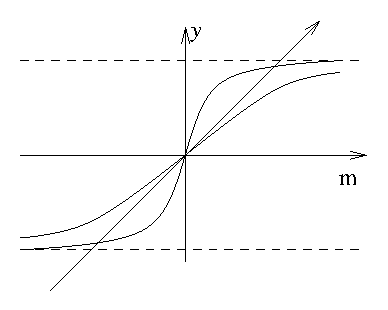
\includegraphics[clip]{1998phy2-1.eps}
   \end{center}
   } 
   \\
   \parbox[t]{60mm}{
   ある$T_c$を境に$m \neq 0$の解が現れる。\\
    $T_c < T$で$m=0$\\
    $T\rightarrow 0$では $\tanh \frac{6Jm}{kT} \rightarrow \pm 1$より\\
    $m \rightarrow \pm 1$\\
    よってグラフは右のようになる。
    }
    \parbox[t]{90mm}{
    
   \begin{center}
    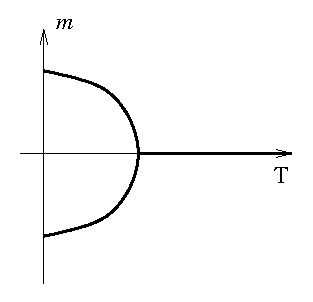
\includegraphics[clip]{1998phy2-2.eps}
   \end{center}
    } 
  \SubSubAnswer
    (ii)より、$h=0$に対して、$m \neq 0$なる解が存在する。$T=T_{\mathrm{c}}$では、
    $\tanh 6 \beta Jm$の$m=0$における傾きが1なので、
\begin{eqnarray}
      T_{\mathrm{c}} = \frac{6J}{k_{\mathrm{B}}} \nonumber
\end{eqnarray}
    である。    
  \end{subsubanswers}
\end{subanswers}



\end{answer}

\end{document}